% !TeX root = ../main.tex

% These appendix images are intentionally placed in a fixed grid instead of separate floating
% figures. Separate floats made LaTeX move almost every screenshot to its own page, while this
% layout keeps the appendix compact and still preserves the figure labels used in the text.
\begin{center}
  \begin{minipage}[t]{0.48\textwidth}
    \centering
    \refstepcounter{figure}\label{fig:timingdata1}
    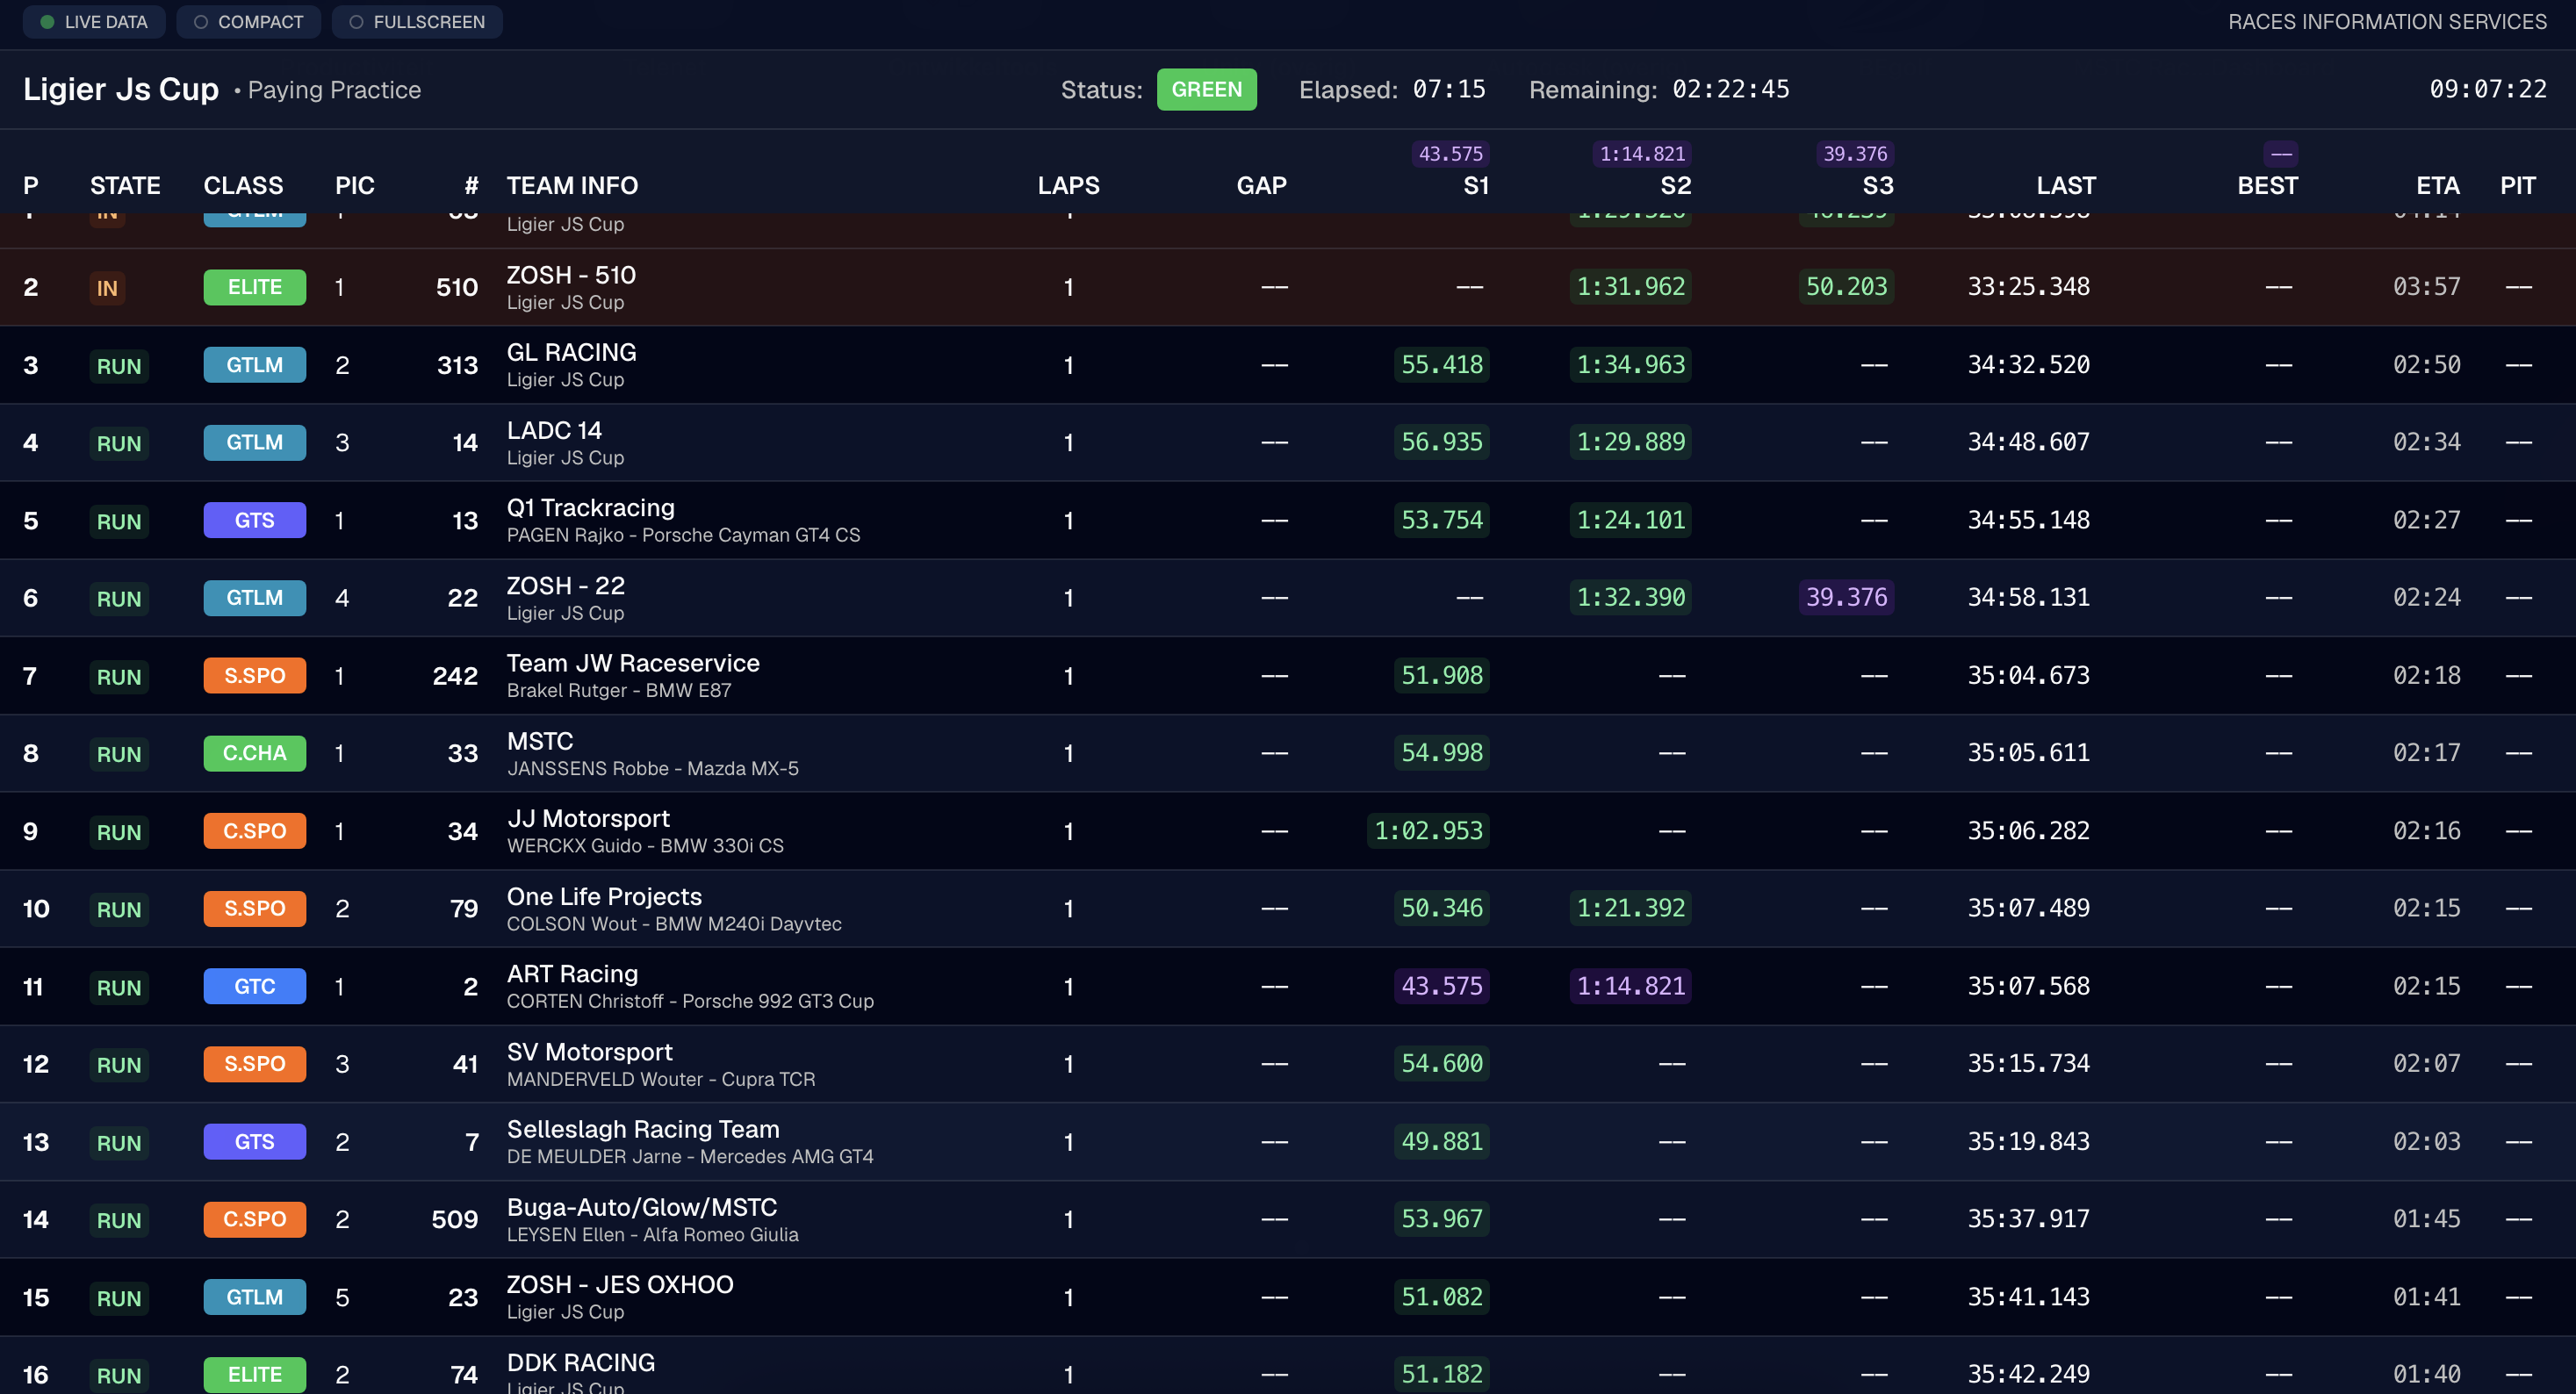
\includegraphics[width=\linewidth]{../figures/timingdata1.png}

    \small\textbf{Figuur~\thefigure:} Screenshot van de officiële timingpagina tijdens de race in
    Spa-Francorchamps. De tabel toont actuele ronde- en sectortijden en maakt zichtbaar hoe
    verschillende klassen door elkaar staan.
  \end{minipage}\hfill
  \begin{minipage}[t]{0.48\textwidth}
    \centering
    \refstepcounter{figure}\label{fig:dashboard-schets1}
    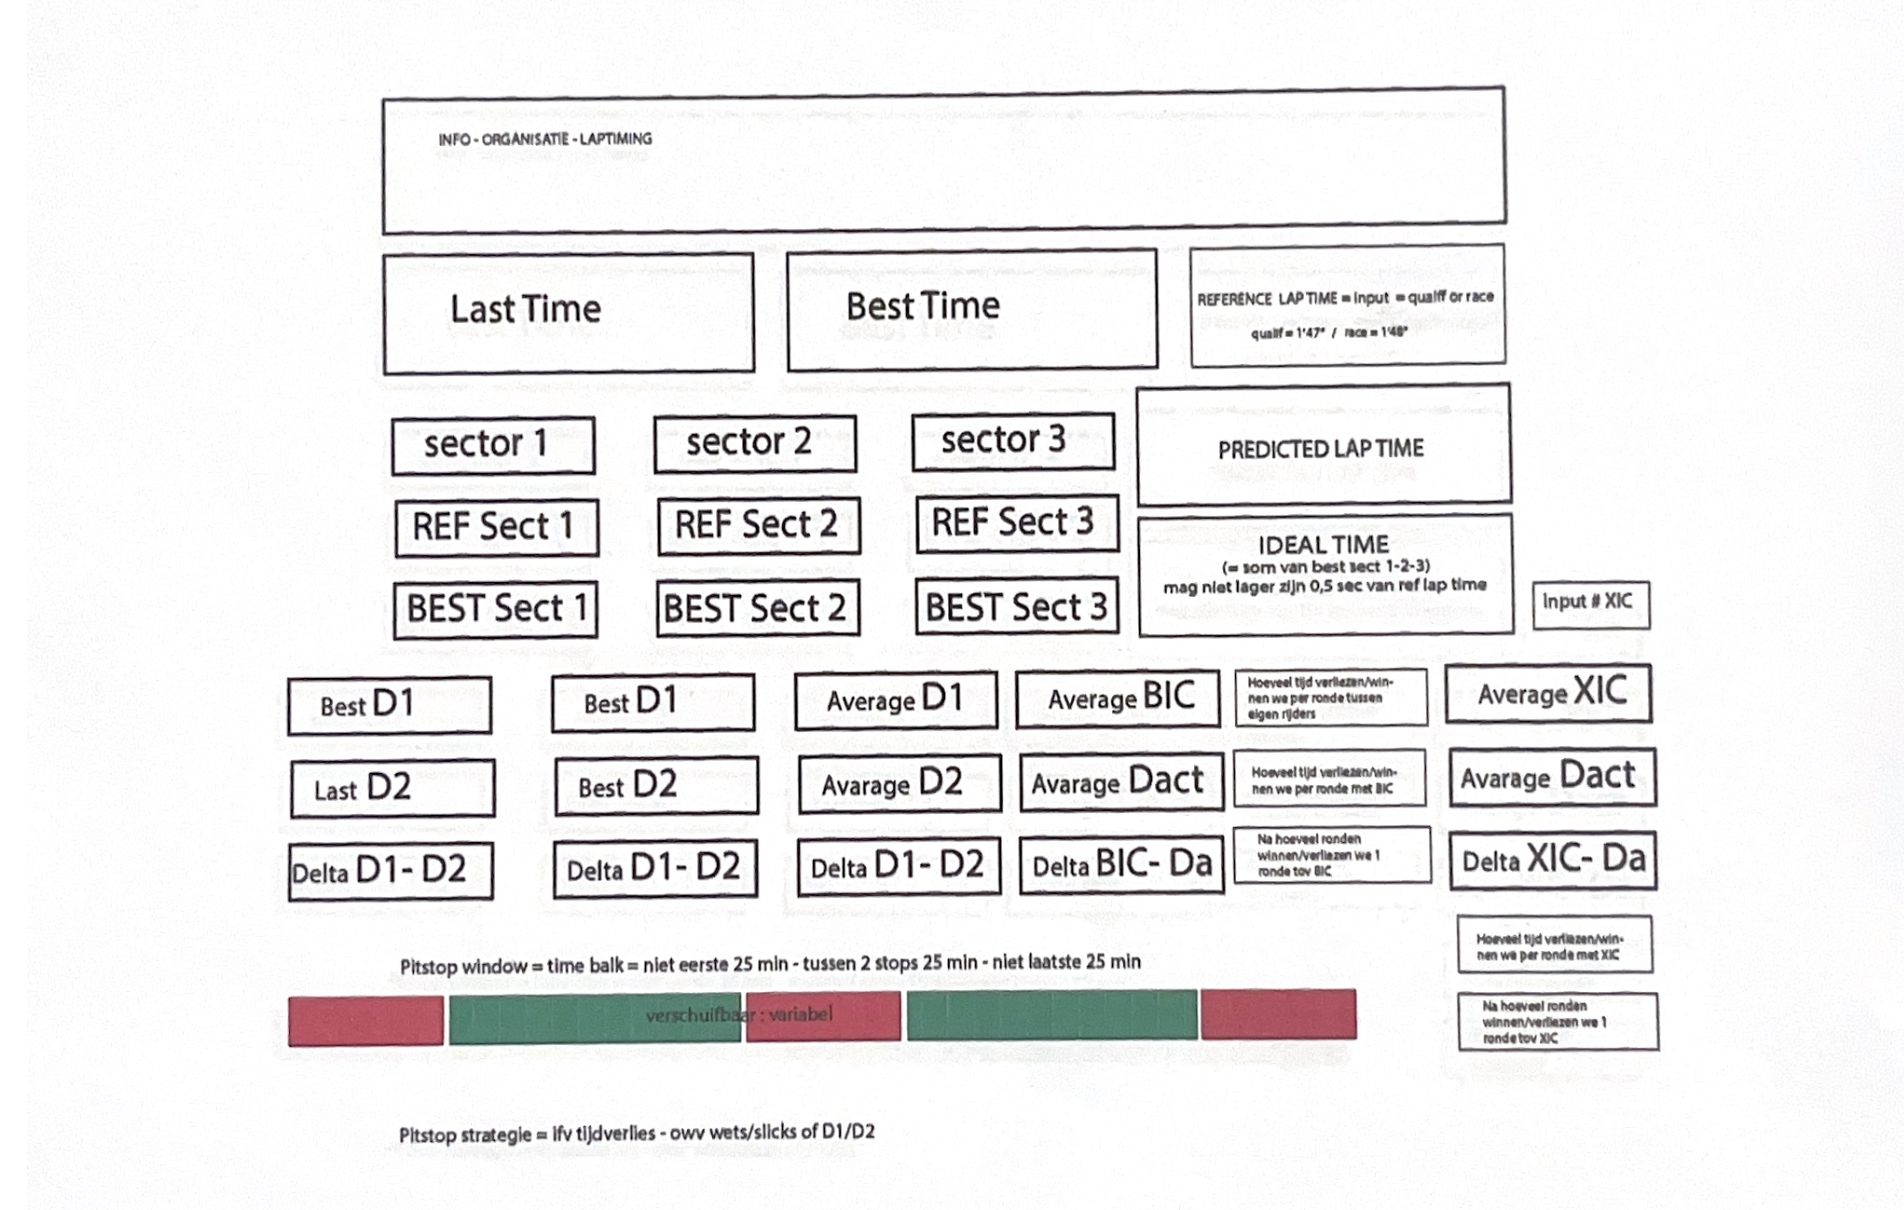
\includegraphics[width=\linewidth]{../figures/dashboard-schets1.png}

    \small\textbf{Figuur~\thefigure:} Schets van het eerste dashboardontwerp. Deze schets werd door
    de opdrachtgever gemaakt en vormde de basis voor de eerste werkende versie.
  \end{minipage}

  \vspace{1.2em}

  \begin{minipage}[t]{0.48\textwidth}
    \centering
    \refstepcounter{figure}\label{fig:versie1}
    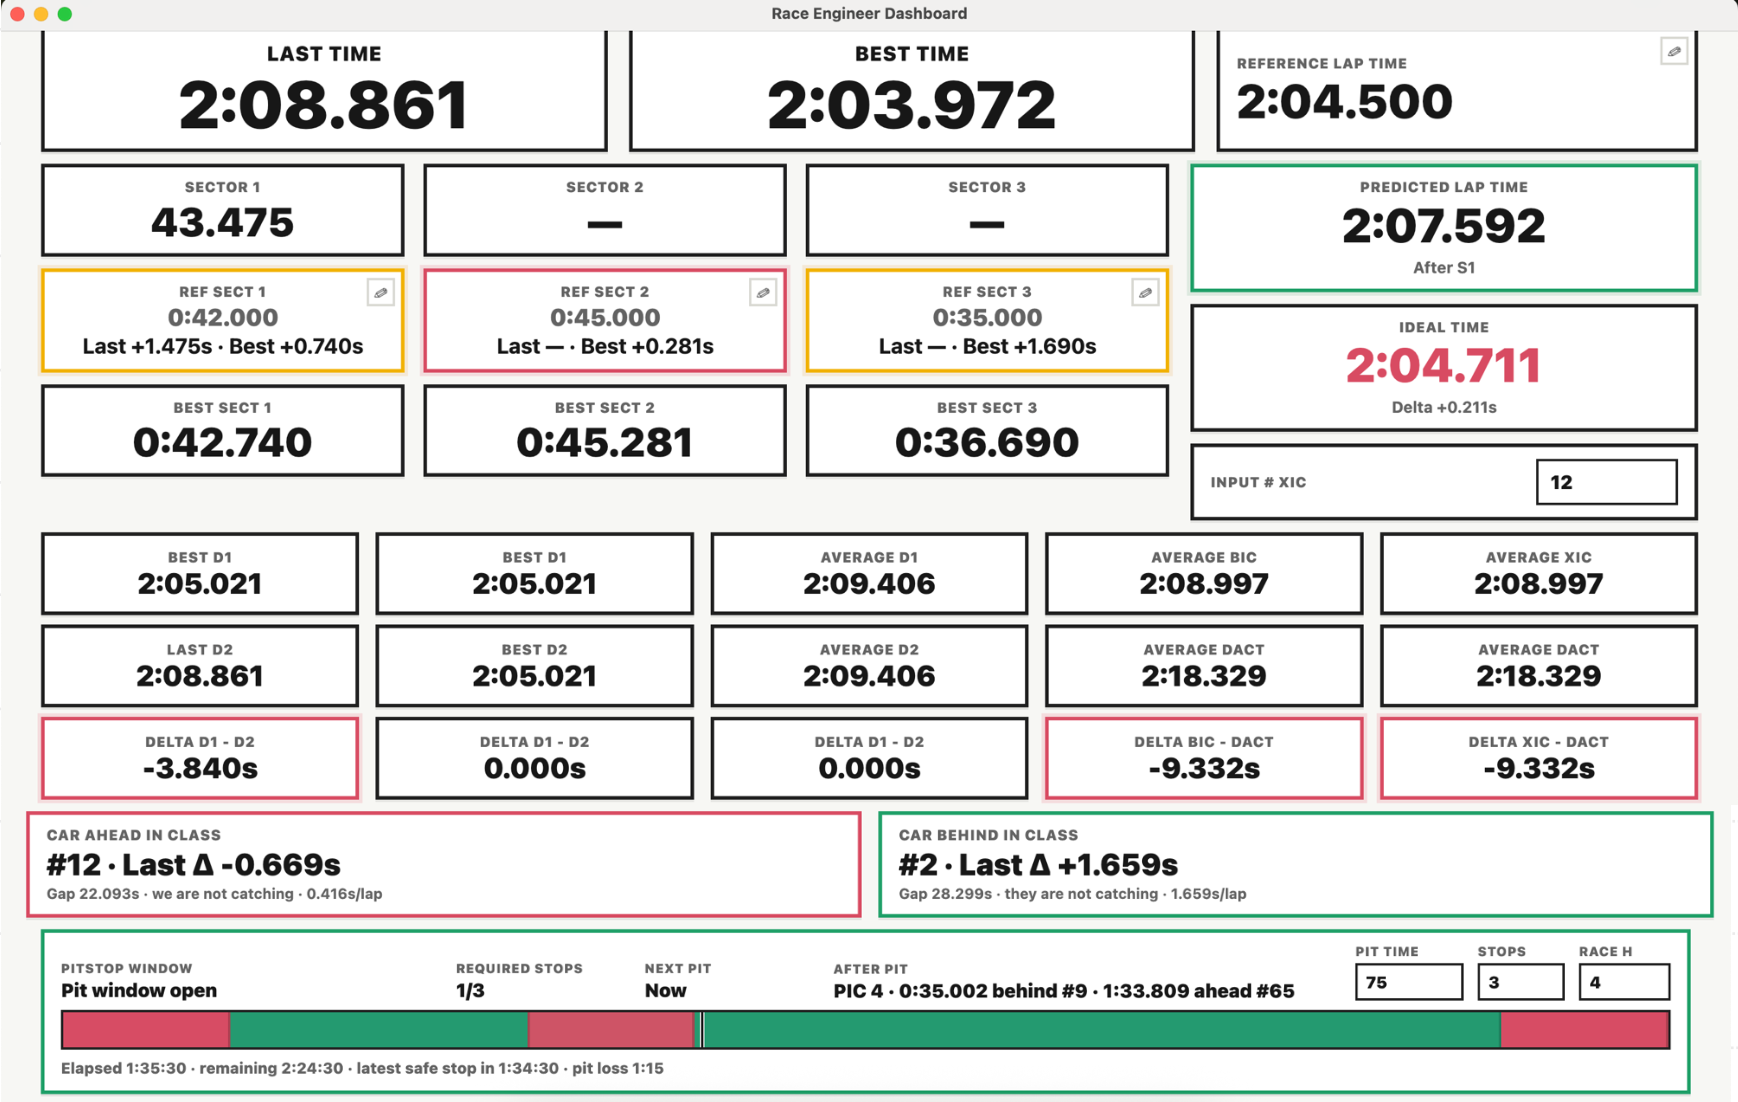
\includegraphics[width=\linewidth]{../figures/versie1.png}

    \small\textbf{Figuur~\thefigure:} Eerste werkende versie van het dashboard, getest tijdens de
    race in Spa-Francorchamps.
  \end{minipage}\hfill
  \begin{minipage}[t]{0.48\textwidth}
    \centering
    \refstepcounter{figure}\label{fig:grafiekvenster1}
    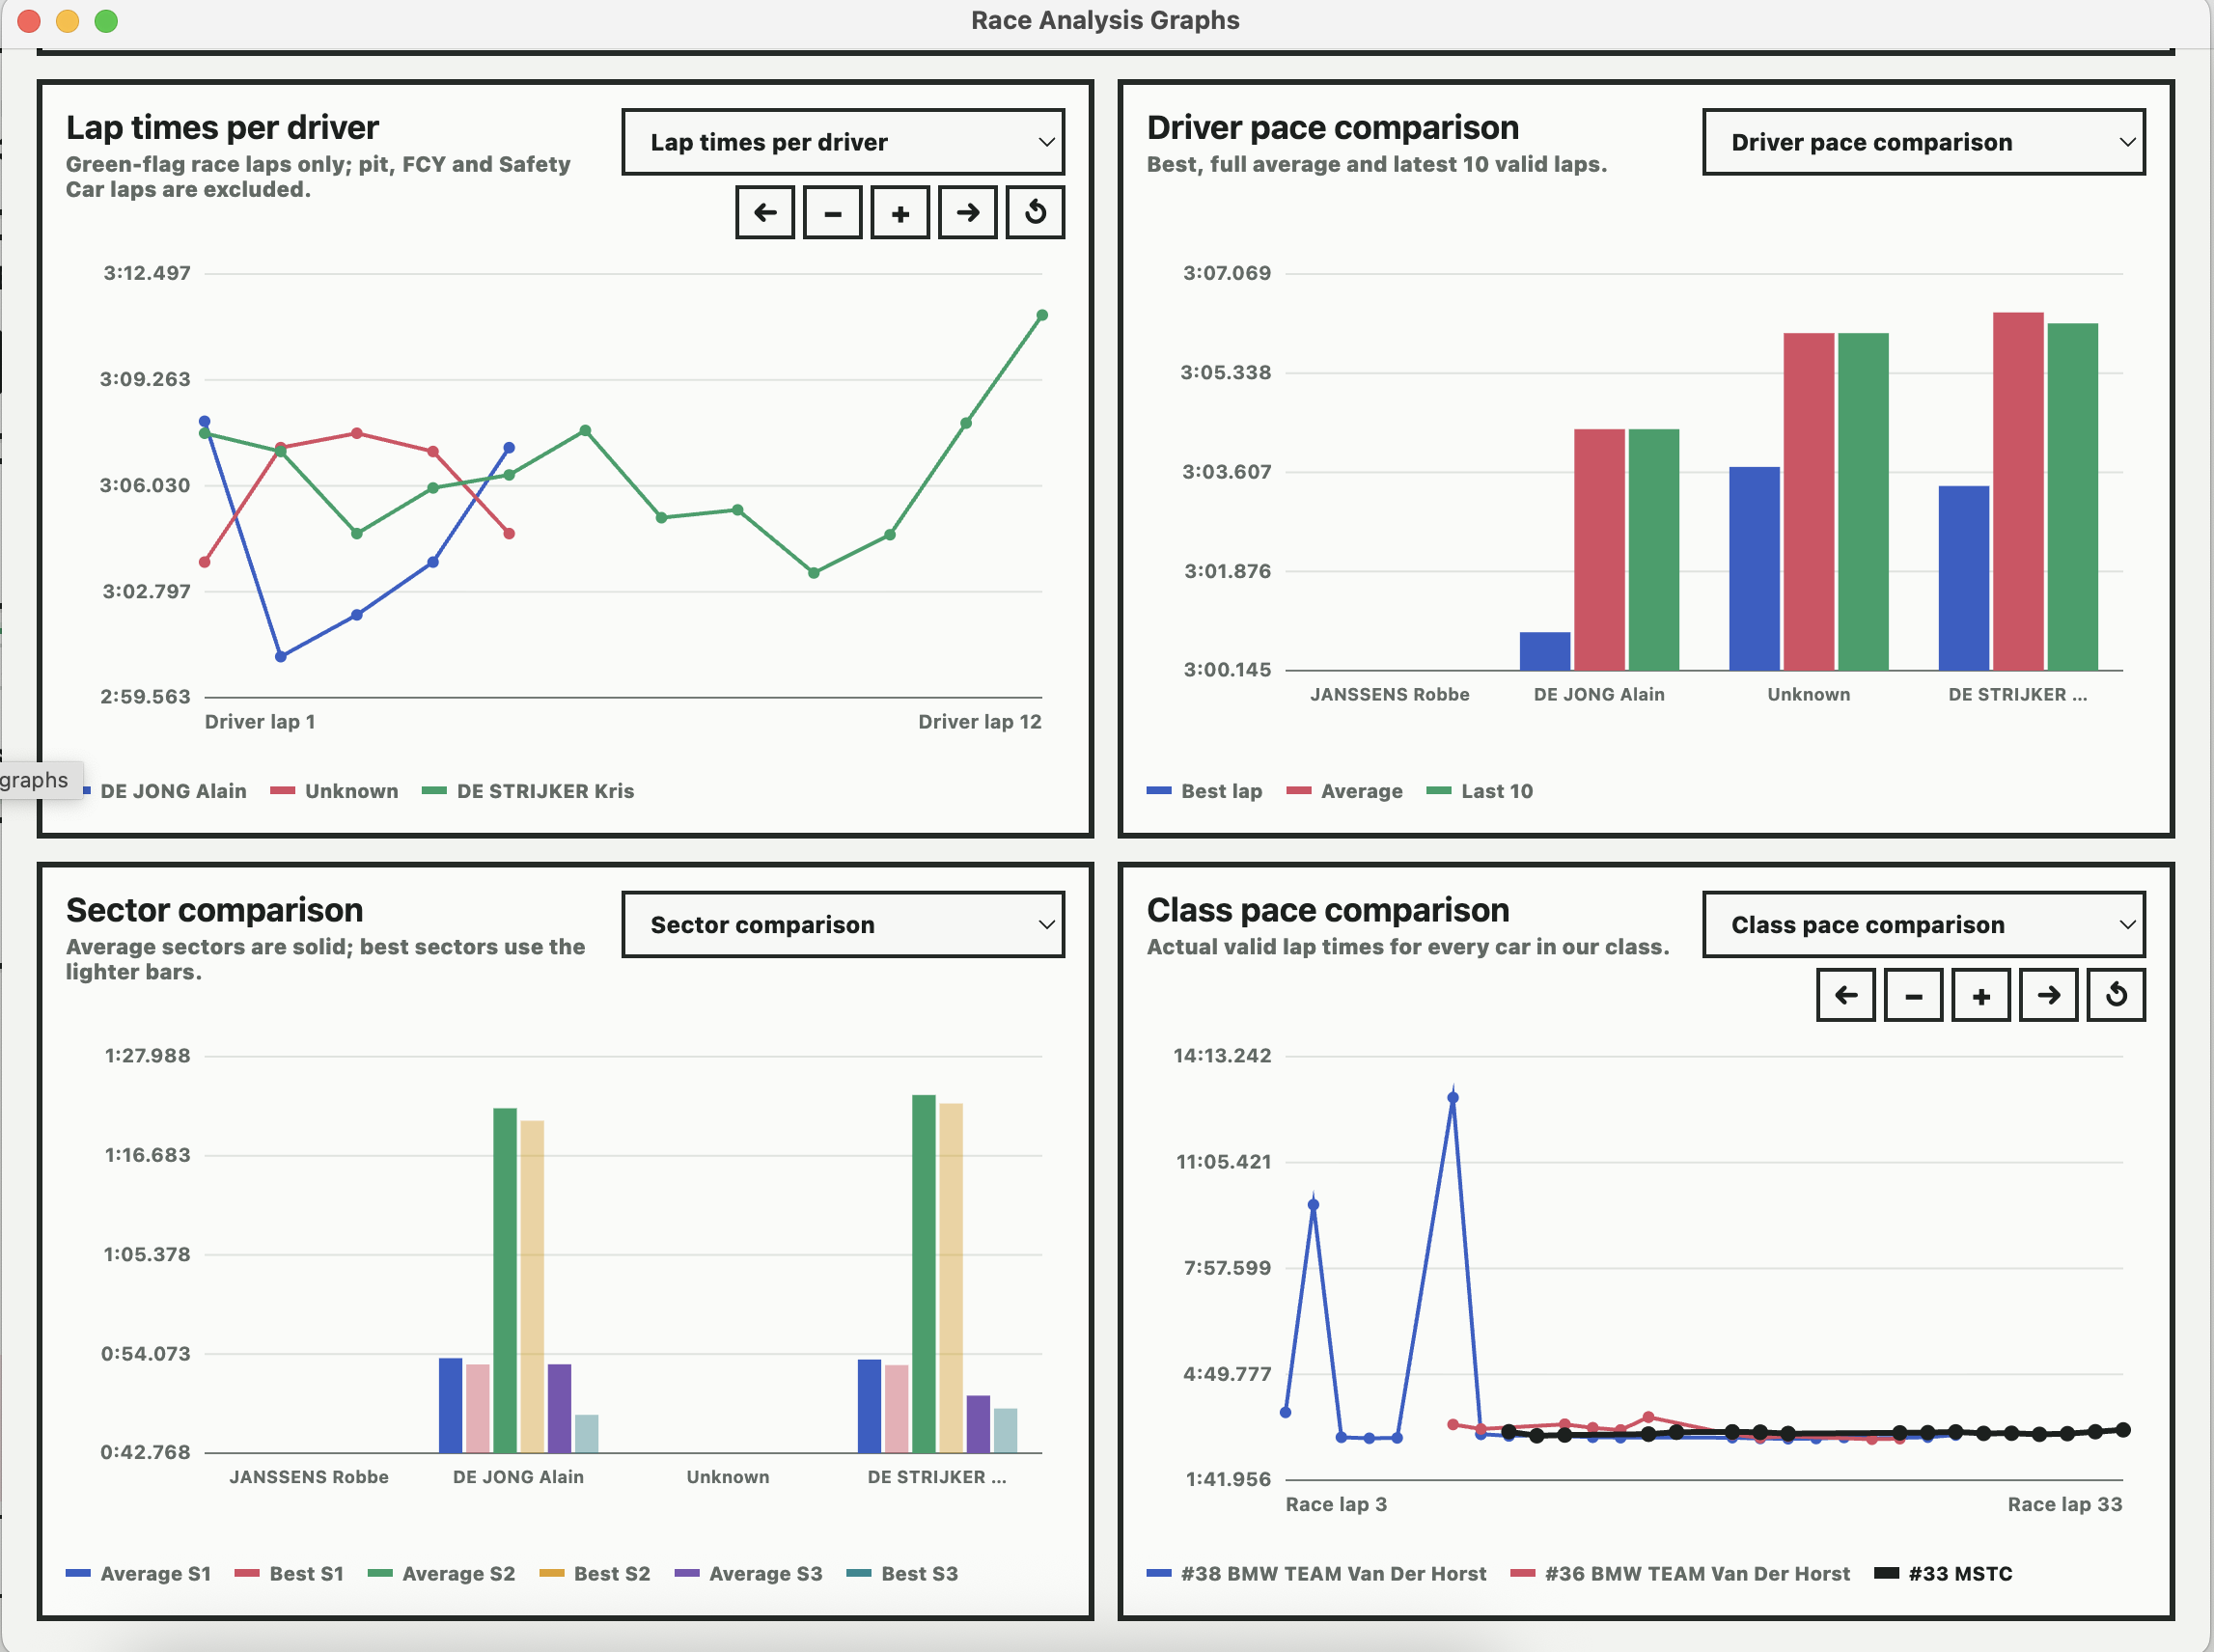
\includegraphics[width=\linewidth]{../figures/grafiekvenster1.png}

    \small\textbf{Figuur~\thefigure:} Eerste werkende grafiekenvenster waarin de evolutie van
    rondetijden en sectoren visueel wordt weergegeven.
  \end{minipage}

  \vspace{1.2em}

  \begin{minipage}[t]{0.48\textwidth}
    \centering
    \refstepcounter{figure}\label{fig:versie1}
    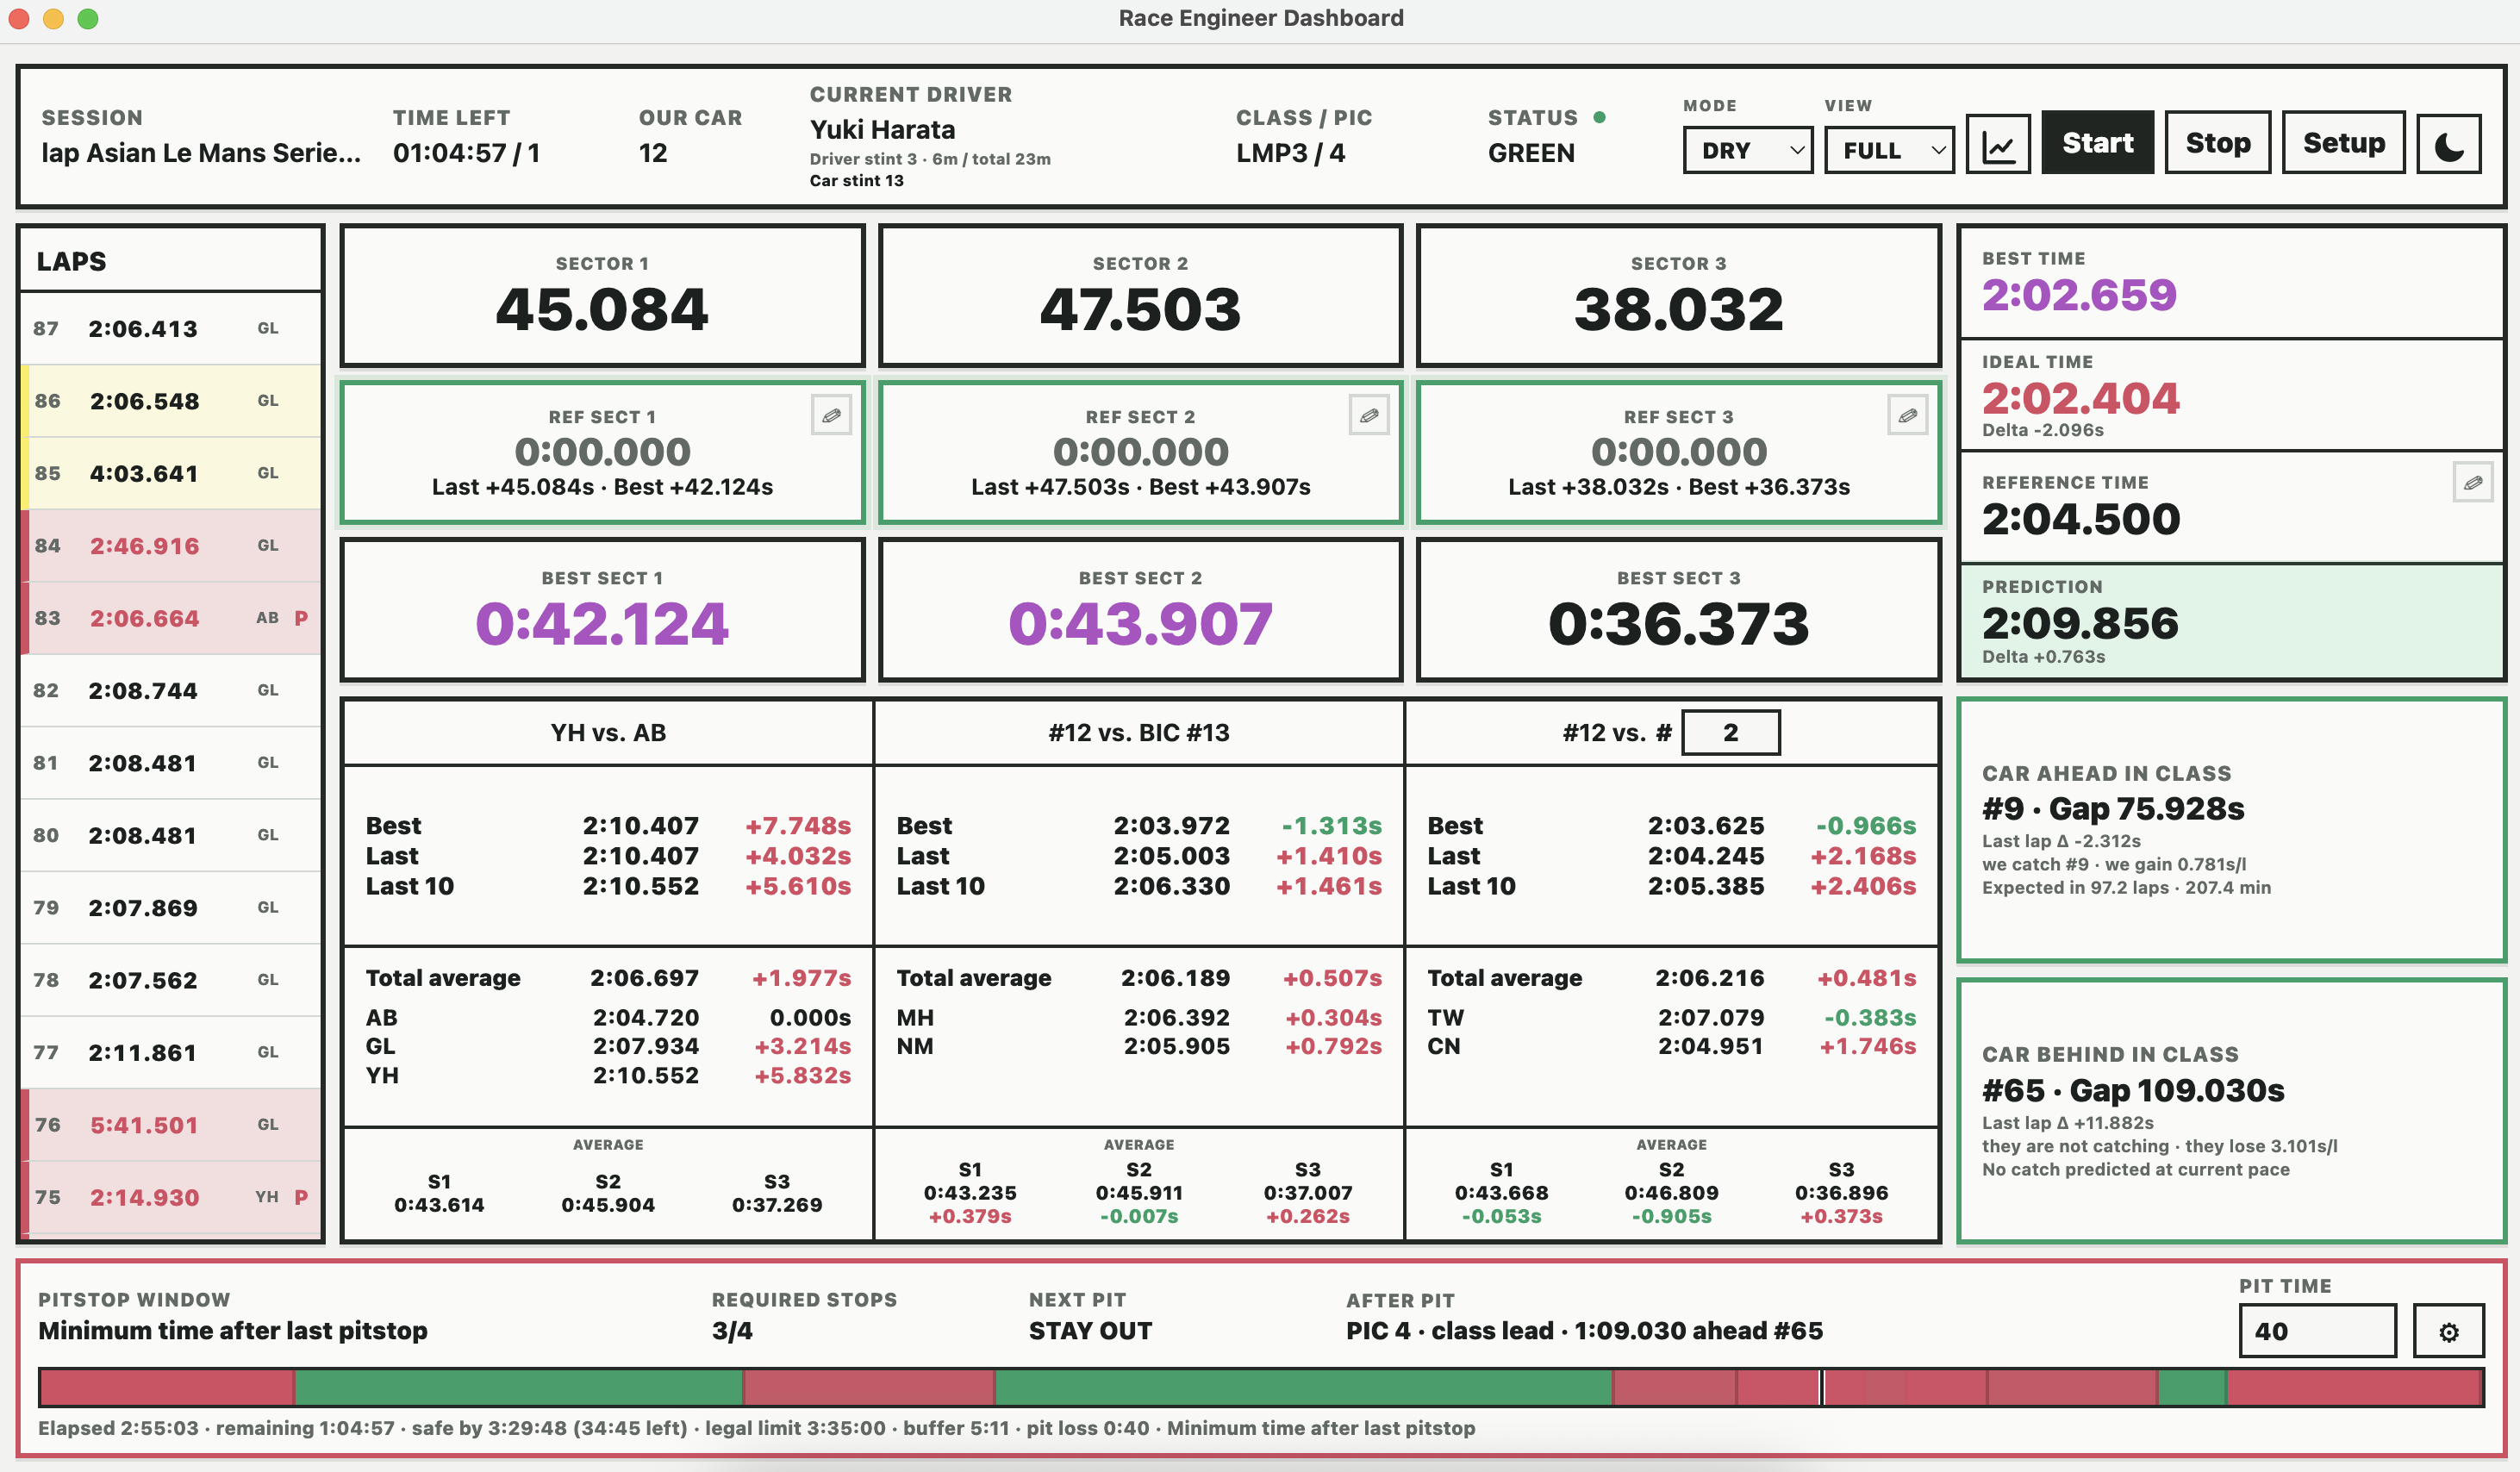
\includegraphics[width=\linewidth]{../figures/final-version.png}

    \small\textbf{Figuur~\thefigure:} Finale versie van het dashboard.
  \end{minipage}\hfill
  
\end{center}
